Before we describe the data-processing stage, let us first give a brief
introduction to the data set that we consider, which is the Google cluster-usage
traces \cite{reiss2011}. The traces were collected over 29 days in May 2011 and
encompass more than 12 thousand machines serving requests from more than 900
users.

In the data set's parlance, a user request is a job; a job comprises one or
several tasks; and a task is a Linux program to be run on a single machine.
Each job is ascribed a unique \up{ID}, and each task is given an \up{ID} that is
unique in the scope of the corresponding job. Apart from other tables, the data
set contains the so-called resource-usage table. The table keeps track of the
resource usage of the tasks with the granularity of five minutes. Each record
corresponds to a specific task and a specific five-minute interval, and it
provides such metrics as the average and maximum values of the \up{CPU}, memory,
and disk usage. There are more than 1.2 billion records, which correspond to
more than 24 million tasks or resource-usage traces and to more than 670
thousand jobs.

The resource-usage table is provided in the form of 500 archives. Each archive
contains a single \up{CSV} file with measurements over a certain time window.
Such a format is inconvenient and inefficient to work with. In particular, in
order to find all the data points that belong to a particular task, one has to
search in all the archives in general. Such a querying strategy is not practical
as reading data is a core operation, which has to be undertaken a myriad of
times during a learning session. The situation is exacerbated further when
multiple learning sessions are to be performed, which is the most common
scenario in practice. All in all, an efficient data-processing pipeline is
needed, which is what we shall develop in this section.

\subsection{Grouping} \slab{grouping}
At the first step, the \up{CSV} data from the 500 archives are distributed into
separate \up{CSV} files so that each such file contains all the data points that
belong to a particular job, resulting in as many \up{CSV} files as there are
jobs. In order to reduce the space requirements, only the used columns of the
table are preserved. In our experiments, these columns are the start time stamp,
job \up{ID}, task \up{ID}, and average \up{CPU} utilization.

Each \up{CSV} file is created and populated in one of a number of folders in
order to reduce the burden on the file system and to have a better organization
in general. To this end, we compute the \up{MD5} hash of the job and task
\up{ID} and use the first letters of the hash as the name of the destination
folder.

Finally, the \up{CSV} files are converted into SQLite databases in order to have
the \up{SQL} language at our disposal for querying the data. In particular, one
has to be able to select only those data points that belong to a particular
task, and the resulting data points have to be ordered chronologically.

\subsection{Indexing} \slab{indexing}
At the second step, an index of the traces is created in order to be able to
efficiently navigate the catalog of the SQLite databases created at the previous
step. Each record in the index contains metadata about a single task, the most
important of which are the task ID and the path to the corresponding SQLite
database. We also include the length of the trace in question into the index in
order to be able to efficiently filter the traces by their lengths at a later
step. The format of the index has been chosen to be \up{CSV}, which is
sufficient in this case, but it can be turned into SQLite if one wishes to store
and subsequently queried more sophisticated metadata than ours.

\subsection{Selection} \slab{selection}
At the last step of our data-processing pipeline, a subset of the resource-usage
traces is selected according to the needs of a learning session using the index
created at the previous step and then stored on the disk. Let us elaborate on
this now.

\begin{figure}[t]
  \centering
  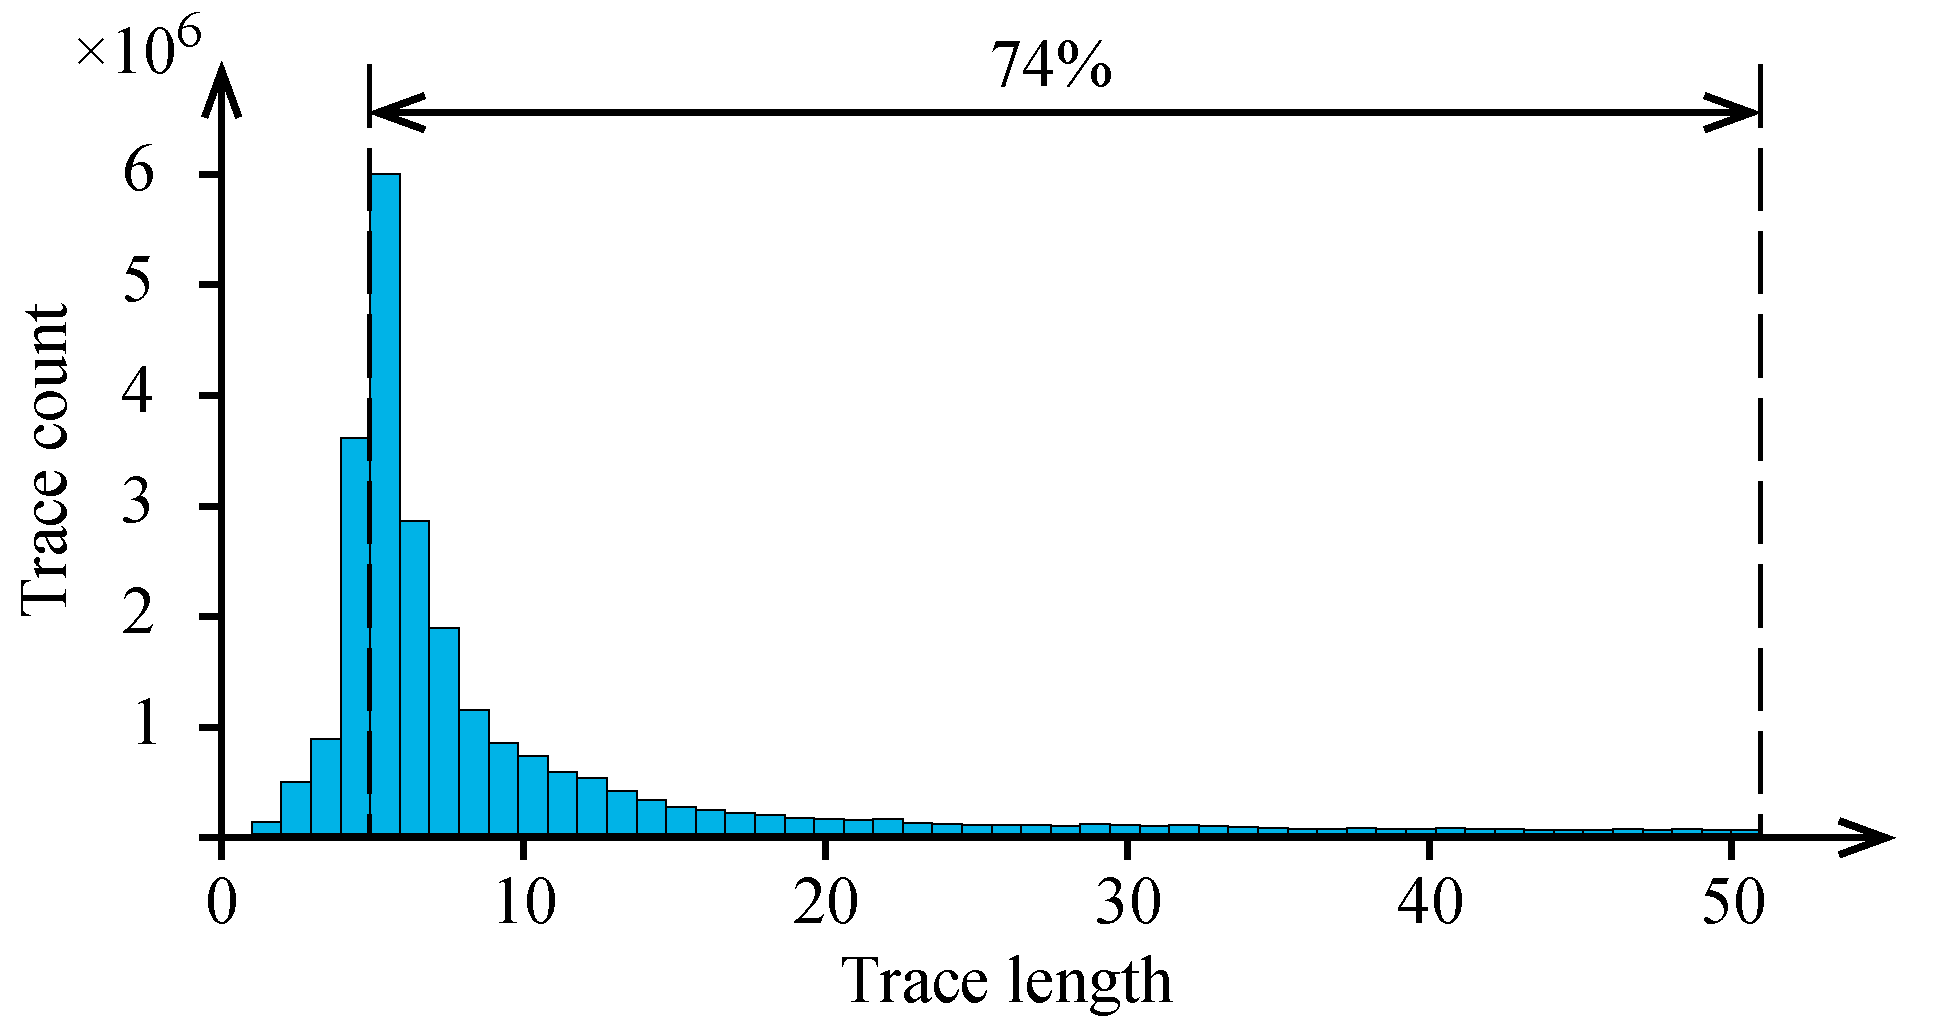
\includegraphics[width=1.0\columnwidth]{include/assets/figures/histogram.pdf}
  \caption{The histogram of the lengths of the resource-usage traces.}
  \flab{histogram}
\end{figure}

First of all, the traces that are too short or too long are filtered out. The
upper bound discards abnormally long traces, which constitute a negligibly small
portion of the data, while the lower one ensures that there is a sufficient
number of data points for the subsequent experimentation. In our experiments, we
focus on those traces that contain 5--50 data points. In other words, we
consider $l_i \in [5, 50]$; recall \eref{trace}. It can be seen in
\fref{histogram}, which shows a truncated histogram of the traces' lengths, that
such traces constitute around 74\% of the total number of traces (around 18 out
of 24 million).

Second of all, we typically work with a random subset of the filtered traces (as
described in the above paragraph). It is typically one or two million
resource-usage traces. By doing so, we obtain shorter development cycles and,
therefore, can iterate on modeling ideas substantially faster. It also makes it
possible to work with the data set on one machine with commodity hardware, which
is what we have at our disposal.

Once the resource-usage traces that will be actually used during a learning
session are known, they are fetched from the corresponding databases and stored
in the native format of the machine-learning library at hand. In our case, this
library is TensorFlow \cite{abadi2015} (to be discussed in \sref{model}), and
the native format is TFRecord. One TFRecord file typically holds multiple
records, which will be then read sequentially, one by one upon request without
clogging memory. Instead of writing all the selected traces into one TFRecord
file, we distribute them across several files relying on \up{MD5} for deciding
on the destination file in a similar way to the one described in
\sref{grouping}. Such a catalog of TFRecord files is created for each of the
three commonly considered parts \cite{hastie2009} of the data at hand: one
catalog is for training, one for validation, and one for testing.

Lastly, it is common practice to standardize data before feeding them into a
machine-learning algorithm \cite{hastie2009}. In our case, it is done along with
creating the aforementioned three catalogs, which requires a separate pass over
the training set.

All the selected and standardized resource-usage traces are denoted by $X$ (see
\sref{problem}), and $X_1$, $X_2$, and $X_3$ will refer to the training,
validation, and testing parts of $X$, respectively.

In conclusion, the benefit of the above pipeline is in the streamlined access to
the data during one or multiple learning sessions. The TFRecord files can be
read efficiently as many times as needed, and they can be straightforwardly
regenerated whenever the selection criteria change; note that the artifacts of
the procedures in \sref{grouping} and \sref{indexing} stay the same. The
presence of multiple TFRecord files allows also for shuffling the training data
at the beginning of each training epoch.

Now we are ready to make use of the obtained data.
